\documentclass{beamer}\usepackage[]{graphicx}\usepackage[]{color}
%% maxwidth is the original width if it is less than linewidth
%% otherwise use linewidth (to make sure the graphics do not exceed the margin)
\makeatletter
\def\maxwidth{ %
  \ifdim\Gin@nat@width>\linewidth
    \linewidth
  \else
    \Gin@nat@width
  \fi
}
\makeatother

\definecolor{fgcolor}{rgb}{0.345, 0.345, 0.345}
\newcommand{\hlnum}[1]{\textcolor[rgb]{0.686,0.059,0.569}{#1}}%
\newcommand{\hlstr}[1]{\textcolor[rgb]{0.192,0.494,0.8}{#1}}%
\newcommand{\hlcom}[1]{\textcolor[rgb]{0.678,0.584,0.686}{\textit{#1}}}%
\newcommand{\hlopt}[1]{\textcolor[rgb]{0,0,0}{#1}}%
\newcommand{\hlstd}[1]{\textcolor[rgb]{0.345,0.345,0.345}{#1}}%
\newcommand{\hlkwa}[1]{\textcolor[rgb]{0.161,0.373,0.58}{\textbf{#1}}}%
\newcommand{\hlkwb}[1]{\textcolor[rgb]{0.69,0.353,0.396}{#1}}%
\newcommand{\hlkwc}[1]{\textcolor[rgb]{0.333,0.667,0.333}{#1}}%
\newcommand{\hlkwd}[1]{\textcolor[rgb]{0.737,0.353,0.396}{\textbf{#1}}}%

\usepackage{framed}
\makeatletter
\newenvironment{kframe}{%
 \def\at@end@of@kframe{}%
 \ifinner\ifhmode%
  \def\at@end@of@kframe{\end{minipage}}%
  \begin{minipage}{\columnwidth}%
 \fi\fi%
 \def\FrameCommand##1{\hskip\@totalleftmargin \hskip-\fboxsep
 \colorbox{shadecolor}{##1}\hskip-\fboxsep
     % There is no \\@totalrightmargin, so:
     \hskip-\linewidth \hskip-\@totalleftmargin \hskip\columnwidth}%
 \MakeFramed {\advance\hsize-\width
   \@totalleftmargin\z@ \linewidth\hsize
   \@setminipage}}%
 {\par\unskip\endMakeFramed%
 \at@end@of@kframe}
\makeatother

\definecolor{shadecolor}{rgb}{.97, .97, .97}
\definecolor{messagecolor}{rgb}{0, 0, 0}
\definecolor{warningcolor}{rgb}{1, 0, 1}
\definecolor{errorcolor}{rgb}{1, 0, 0}
\newenvironment{knitrout}{}{} % an empty environment to be redefined in TeX

\let\hlesc\hlstd \let\hlpps\hlstd \let\hllin\hlstd \let\hlslc\hlcom \let\hlppc\hlcom
\usepackage{alltt}

%normal
\usepackage{color}
\usepackage{beamerthemebars}
\usepackage{lmodern}
\usepackage{multicol}

\usetheme{AnnArbor}
\usecolortheme{wolverine}

%redefined colors for beamer
\definecolor{beamer@UIUCblue}{RGB}{0,60,125}
\definecolor{beamer@UIUCorange}{RGB}{244,127,36}
% taken from 
% http://identitystandards.illinois.edu/graphicstandardsmanual/generalguidelines/colors.html

\definecolor{beamer@UIUCgray}{RGB}{210,210,210}
%warning text
\definecolor{customgreen}{RGB}{2,103,1}

\setbeamercolor{frametitle}{fg=beamer@UIUCblue,bg=beamer@UIUCgray}
\setbeamercolor{normal text}{fg=black}
\setbeamercolor{title}{fg=beamer@UIUCblue,bg=beamer@UIUCorange}
\setbeamercolor{item projected}{fg=white,bg=beamer@UIUCorange}
%boxes
\setbeamercolor{block title}{fg=beamer@UIUCblue,bg=beamer@UIUCorange}
\setbeamercolor{block body}{fg=blue,bg=beamer@UIUCblue!80}
\setbeamercolor{title in head/foot}{fg=beamer@UIUCblue,bg=beamer@UIUCgray}
\setbeamercolor{author in head/foot}{fg=white,bg=beamer@UIUCblue}
\setbeamercolor{institute in head/foot}{fg=white,bg=beamer@UIUCorange}
\setbeamercolor{date in head/foot}{fg=white,bg=beamer@UIUCorange}
\setbeamercolor{section in head/foot}{fg=white,bg=beamer@UIUCblue}
\setbeamercolor{subsection in head/foot}{fg=white,bg=beamer@UIUCorange}

%override title link color
\makeatletter
\renewcommand\insertshorttitle[1][]{%
  \beamer@setupshort{#1}%
  \let\thanks=\@gobble%
  \ifnum\c@page=1%
  \hyperlinkpresentationend{\beamer@insertshort{\usebeamercolor*[fg]{title in head/foot}\beamer@shorttitle}}%
  \else%
  \hyperlinkpresentationstart{\beamer@insertshort{\usebeamercolor*[fg]{title in head/foot}\beamer@shorttitle}}%
  \fi}
\makeatother

\usepackage{etoolbox}
\makeatletter
\patchcmd{\beamer@section}
  {\def\insertsectionhead{\hyperlink{Navigation\the\c@page}{#1}}}
  {\def\insertsectionhead{\hyperlink{Navigation\the\c@page}{\usebeamercolor*[fg]{section in head/foot}#1}}}
  {}{}
\patchcmd{\beamer@subsection}
  {\def\insertsubsectionhead{\hyperlink{Navigation\the\c@page}{#1}}}
  {\def\insertsubsectionhead{\hyperlink{Navigation\the\c@page}{\usebeamercolor*[fg]{subsection in head/foot}#1}}}
  {}{}
\makeatother


%insert timeline
\AtBeginSection[]
{
  \begin{frame}
    \frametitle{On the Agenda}
    \begin{multicols}{2}
    \tableofcontents[currentsection]
    \end{multicols}
  \end{frame}
}


%\setbeamercolor{palette tertiary}{bg=beamer@UIUCblue,fg=white}
%\setbeamercolor{palette secondary}{bg=beamer@UIUCgray,fg=white}
%\setbeamercolor{palette primary}{bg=beamer@UIUCorange,fg=white}

\beamertemplatenavigationsymbolsempty %hides navigation.
\usepackage{graphicx}
\usepackage{comment}
\usepackage{hyperref}
\hypersetup{colorlinks=true,urlcolor=beamer@UIUCblue,linkcolor=beamer@UIUCblue,% link color controls section, subsection, and title
citecolor = beamer@UIUCorange,
anchorcolor = beamer@UIUCorange}
\usepackage{amssymb,amsmath}
\usepackage{multirow}
\usepackage{upgreek}

%flow charts
\usepackage{tikz}
\usetikzlibrary{shapes,arrows}

\author[J Balamuta]{James Balamuta}
\institute[UIUC]{Department of Statistics \\
University of Illinois at Urbana-Champaign \\
\href{mailto:balamut2@illinois.edu}{\nolinkurl{balamut2@illinois.edu} }}





\IfFileExists{upquote.sty}{\usepackage{upquote}}{}
\begin{document}


\date[STAT 385]{\today \\ Department of Statistics}

\title[Reproducible Research]{
\begin{columns}
\column{.15\textwidth}
\hspace{.2in}
\vspace{.1in}

\includegraphics{imark_bold-eps-converted-to.pdf}
\column{.85\textwidth}
{Reproducible Research via R, \LaTeX, and knitr}
\end{columns}
}
\frame{\titlepage}

\begin{frame}
\frametitle{On the Agenda}   
\begin{multicols}{2}
\tableofcontents[]
\end{multicols}
\end{frame}

\begin{frame}
\begin{center}
\Huge Ready?
\end{center}
\end{frame}

\section{Reproducible Research}
\subsection{Definition}
\begin{frame}
        \frametitle{What is Reproducible research?}
        \textbf{Reproducible Research} is the idea that the experiment's collected data, data analysis code, and derived principal results are assembled in a way so that another body is able to re-create all of the results (e.g., data formatting, parameter estimates, figures, tables, and so on ). 
        \\$ $\\
        In essence, reproducible research seeks to satisfy a very minimal portion of how to obtain \textit{replicable} results championed by the scientific theory. 
\end{frame}


\begin{frame}
\frametitle{Reproducible vs. Replicable}
In general, there are \href{http://cogprints.org/7691/7/ICMLws09.pdf}{lots} of \href{http://magazine.amstat.org/blog/2011/07/01/trust-your-science/}{papers} that debate what the definitions of Reproducible and Replicable are. 
\\$ $\\
For our purpose, we will consider the viewpoint of \href{http://www.sciencemag.org/content/334/6060/1226.full}{Prof. Roger Peng of the Journal of Biostatistics} - held as the \href{http://biostatistics.oxfordjournals.org/content/10/3/405.full}{Journal's standard} - and \href{http://bioinformatics.mdanderson.org/Supplements/ReproRsch-All/Modified/ENAR/banksNotes.pdf}{echoed by Prof. David Banks}, former editor of JASA.
\\$ $\\
\begin{description}
\item[Reproducible] if there is a specific set of computational functions/analyses (usually specified in terms of code) that exactly reproduce all of the numbers in a published paper from raw data.
\item[Replicable] if you perform the exact same experiment (at least) twice, collect data in the same way both times, perform the same data analysis, and arrive at the same conclusions. 
\end{description}
\end{frame}

\begin{frame}
\frametitle{Why Practice Reproducible Research?}
Many issues have arisen over the recent years regarding the validity of the results published in Journals. 
\\$ $\\
By structuring research so that it is reproducible, not only is the work more useful and acceptable to Journals but also the overload on the researcher is reduced.
\\$ $\\
The overload is reduced since the hope of reproducible research is to put an end to the practice of copying and pasting results into documents, asymmetric data modifications in excel, and undocumented code.
\\$ $\\
As they say...
\\
If you do something \textit{by hand} once, you'll end up doing it at least 20 times.
\end{frame}

\tikzstyle{decision} = [diamond, draw, fill=beamer@UIUCorange!60, 
    text width=5.5em, text badly centered, node distance=3.5cm, inner sep=0pt]
\tikzstyle{block} = [rectangle, draw, fill=beamer@UIUCblue!60, 
    text width=5em, text centered, rounded corners, minimum height=4em, node distance=3.5cm]
\tikzstyle{block2} = [rectangle, draw, fill=beamer@UIUCblue!60, 
    text width=11em, text centered, rounded corners, minimum height=4em, node distance=3cm]
\tikzstyle{line} = [draw, -latex']
\tikzstyle{cloud} = [draw, ellipse,fill=red!20, node distance=3.5cm,
    minimum height=2em]

\subsection{Workflow}
\begin{frame}
\frametitle{Ideal Work Flow}
\begin{tikzpicture}[node distance = 2cm, auto, scale=0.75, every node/.style={scale=0.75}]
    % Place nodes
    \node [cloud] (raw) {Raw Data};
    \node [block, right of=raw] (format) {Import and Clean Data};
    \node [block, right of=format] (analysis) {Data Analysis};
    \node [decision, right of=analysis] (presentation) {Presentation};
    \node [block2, above of=presentation] (latex) {\LaTeX $\,$  via .Rnw \\
                                                  (Article, Book, Beamer)}; 
    \node [block2, below of=presentation] (markdown) {RMarkdown   via .Rmd \\
                                                     (HTML, Presentations)}; 

    % Draw edges
    \path [line, dashed] (raw) -- (format);
    \path [line] (format) -- (analysis);
    \path [line] (analysis) -- (presentation);
    \path [line] (presentation) -- (latex);
    \path [line] (presentation) -- (markdown);
\end{tikzpicture}

Only raw data exists outside of the ecosystem. 
\\
All blue boxes are done with a script to ensure reproducibility.
\end{frame}


\tikzstyle{decision} = [diamond, draw, fill=beamer@UIUCorange!60, 
    text width=5.5em, text badly centered, node distance=5cm, inner sep=0pt]
\tikzstyle{block} = [rectangle, draw, fill=beamer@UIUCblue!60, 
    text width=5em, text centered, rounded corners, minimum height=4em, node distance=5.5cm]

\begin{frame}
\frametitle{The Power of Scripts}

\begin{tikzpicture}[node distance = 2cm, auto, scale=0.85, every node/.style={scale=0.85}]
    % Place nodes
    \node [block] (format) {Import and Clean Data};
    \node [block, right of=format] (analysis) {Data Analysis};
    \node [decision, right of=analysis] (presentation) {Presentation};

    % Draw edges
    \path [line] (format) -- (analysis);
    \path [line] (analysis) -- (presentation);
\end{tikzpicture}

\begin{columns}[t]
\onslide<1->{
\begin{column}{0.33\textwidth}
\centering
\begin{itemize}
\item Modifications are documented
\item Uniformly applied cleaning methods
\item Resiliency to wrong data version 
\end{itemize}
\end{column}}
\onslide<1->{
\begin{column}{0.33\textwidth}
\begin{itemize}
\item Perform analysis like normal, but...
\item No need to export figures or tables
\item Code is \textbf{reusable} between projects
\end{itemize}
\end{column}}
\onslide<1->{
\begin{column}{0.33\textwidth}
\begin{itemize}
\item Figures and tables are already created!
\item Analysis changed? \textbf{Auto-updates!}
\item Results are shareable and customizable
\end{itemize}
\end{column}}
\end{columns}
\end{frame}

\begin{frame}
\frametitle{The Best Reason to Practice Reproducible Research...}
\centering
\LARGE
Chances are your closest collaborator is yourself from three months ago, who conveniently does not reply to emails.
\end{frame}

\section{Tools of Reproducible Research}
\subsection{Overview}
\begin{frame}
\frametitle{Software of Reproducible Research}
The following software programs are key to Reproducible Research:
\begin{itemize}
  \item \href{http://cran.r-project.org/}{R} - Programming Language
  \item \href{http://rstudio.com/ide/download}{R Studio} - Integrated Developer Environment for R 
  \item \href{http://latex-project.org/ftp.html}{\LaTeX} - Your Favoriate Distribution of \LaTeX
  \item \href{https://github.com/jgm/pandoc/releases}{pandoc} - Swiss Army Knife of Document Conversion
  \item \href{http://git-scm.com/downloads}{git} - Version Control System (VCS)
\end{itemize}
\end{frame}

\begin{frame}
\frametitle{R Packages used in Reproducible Research}
Within R, there are several packages oriented at enabling Reproducible Research. The list below is not extensive. For more options, see the \href{http://cran.r-project.org/web/views/ReproducibleResearch.html}{CRAN Task View on Reproducible Research}.
\\$ $\\
For the presentation, I will focus on the following R packages:
\begin{itemize}
  \item \href{http://yihui.name/knitr/demos}{knitr} - Dynamic Report Generation
  \item \href{http://cran.r-project.org/web/packages/rmarkdown/index.html}{rmarkdown} - R interface to Pandoc
\end{itemize}

\end{frame}

\subsection{Setting up the Workspace}

\begin{frame}[fragile]
\frametitle{Configuring RStudio to build \texttt{knitr} documents}
 Make sure that \texttt{knitr} is install before continuing (install.packages("knitr"))
\begin{columns}[t]
\column{.36\textwidth}
\centering
\begin{block}{Click \texttt{`Tools'} \\ Select \texttt{`Global Options'}}
\centering
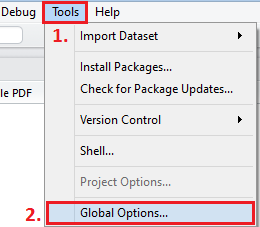
\includegraphics[scale=0.5]{img/configrstudio_opt.png}
\end{block}
\column{.53\textwidth}
\centering
\begin{block}{Click \texttt{`Sweave'} \\ Select \texttt{`knitr'} from drop down menu}
\centering
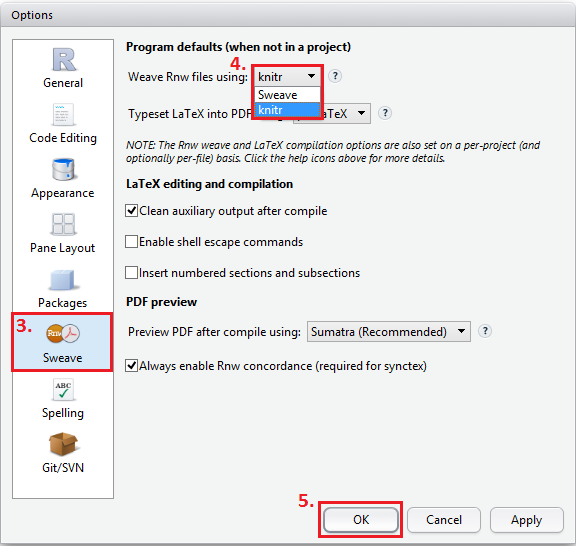
\includegraphics[scale=0.34]{img/set_to_knitr.png}
\end{block}
\end{columns}
\end{frame}

\begin{frame}
\frametitle{Initializing the Workspace} 

The Checklist:
\begin{enumerate}
\item Make sure everything is up-to-date (R, R Studio, and R Packages)
\begin{itemize}
\item Depending on how sensitive the analysis is, consider using \href{http://cran.r-project.org/web/packages/packrat/index.html}{packrat} to create project based libraries for r packages.
\end{itemize}
\item Create a repository on \href{http://github.com}{GitHub}
\item Setup an R project in R Studio based on the repository.
\item Place project directory in either \href{www.dropbox.com}{Dropbox} or \href{https://app.box.com/}{BoxSync} folder.
\begin{itemize}
\item Make sure to turn off new file notification... 
\end{itemize}
\end{enumerate}

\end{frame}

\begin{frame}
\frametitle{STATS@UIUC Analytical Environment}
Starting in the \textbf{Spring of 2016}, the Department of Statistics at the University of Illinois has had an online analytical environment. The primary purpose of this analytical environment is to try out various approaches to working with technology in Statistics.
\\$ $

{\Large
\centering
\url{https://rstudio.stat.illinois.edu}
}
$ $\\$ $\\
To login, please use your NetID and Active Directory Password or what you use to log into \href{https://compass2g.illinois.edu}{Compass2g}. 
\\$ $\\$ $\\ 
The instructions given next are for users who opt to use their own computer instead of the platform.
\end{frame}

\begin{frame}[fragile]
\frametitle{Obtaining git on Windows}

Unfortunately, unlike macOS and Linux, Windows does not currently have native support for git. This will change when \texttt{bash} is added to the command line.
\\$ $\\
Until then, to have \texttt{git} on your system you must download it from \url{http://git-scm.com/downloads}.
\\$ $\\
Furthermore, during the installation, \textbf{make sure you select the option that places git.exe on your system's PATH variable.} 
\\$ $\\$ $\\
Both of these steps are omitted here.
\end{frame}

\begin{frame}[fragile]
\frametitle{Configuring git for the first time}

Once git is installed, you will have to provide an initial configuration scheme.

\begin{columns}[t]
\column{.36\textwidth}
\centering
\begin{block}{Open Git Bash from Start Menu}
\centering

\includegraphics[scale=0.32]{img/git/select_git_bash.png}
\end{block}
\column{.53\textwidth}
\centering
\begin{block}{Enter the following two commands using your information}
\centering
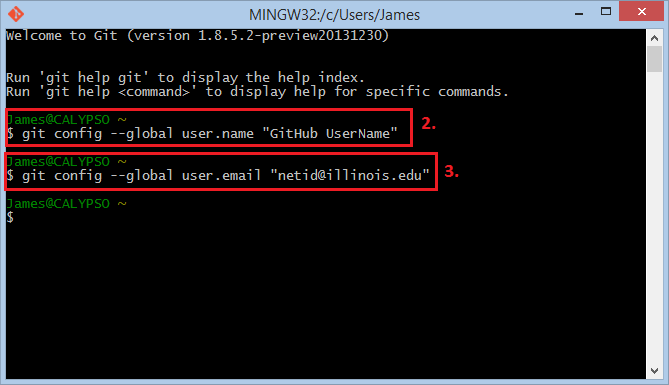
\includegraphics[scale=0.36]{img/git/git_global_config.png}
\end{block}
\end{columns}

\end{frame}


\begin{frame}
\frametitle{Create a GitHub Account}

Register an account on \href{http://github.com}{GitHub} using your @illinois.edu e-mail address.
\begin{center}

\includegraphics[scale=0.32]{img/git/github_reg.png}
\end{center}

\end{frame}

\begin{frame}
\frametitle{Request a Student Account}

Place a request using \href{https://education.github.com/discount_requests}{GitHub Education} to obtain \textbf{unlimited} free private repositories. Also, consider forming an organization, which is able to receive \textbf{unlimited} free private repositories with fine permission control. 
\begin{center}

\includegraphics[scale=0.23]{img/git/ed_discount.png}
\end{center}

\end{frame}

\begin{frame}
\frametitle{BitBucket: An alternative to GitHub}

Dislike GitHub? Consider using \href{https://bitbucket.org/}{BitBucket}. The repositories are generally more closed source than GitHub. However, for researchers and students, BitBucket provides \href{https://www.atlassian.com/software/views/bitbucket-academic-license.jsp}{unlimited private repositories with unlimited contributors}.
\begin{center}
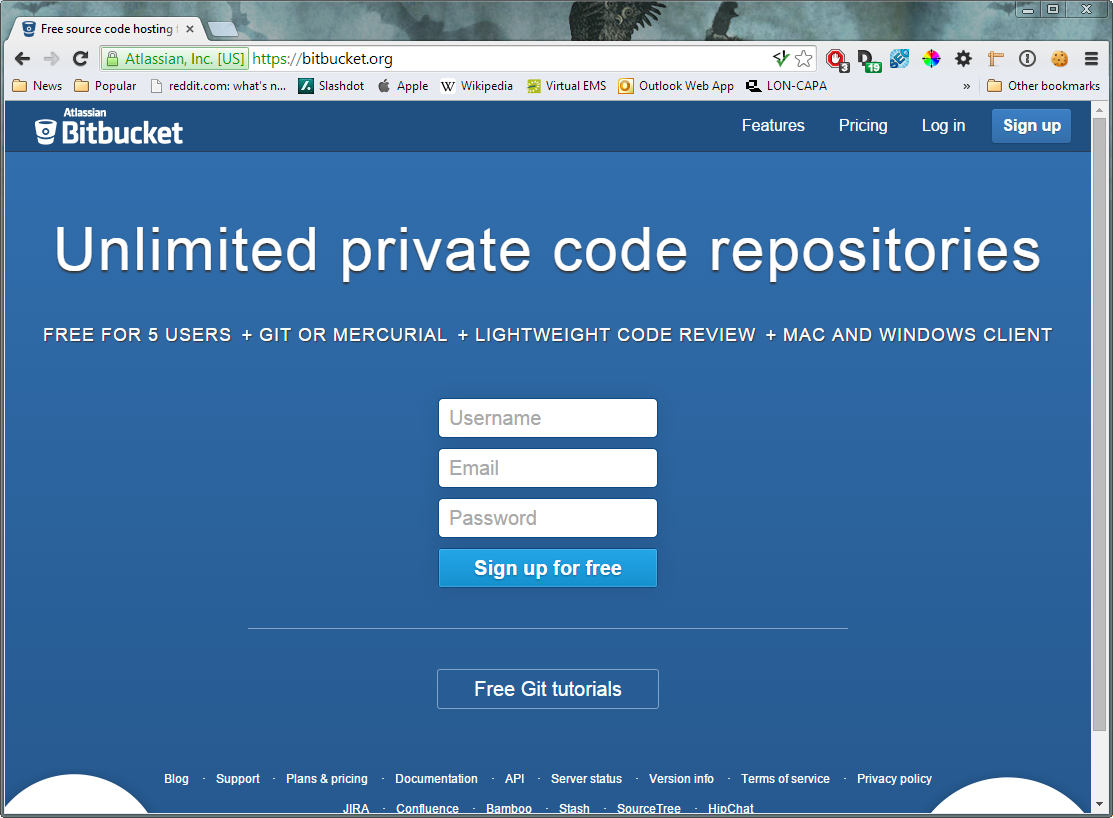
\includegraphics[scale=0.25]{img/git/bitbucket_reg.png}
\end{center}

\end{frame}


\begin{frame}
\frametitle{Create a GitHub Repository}

\begin{center}
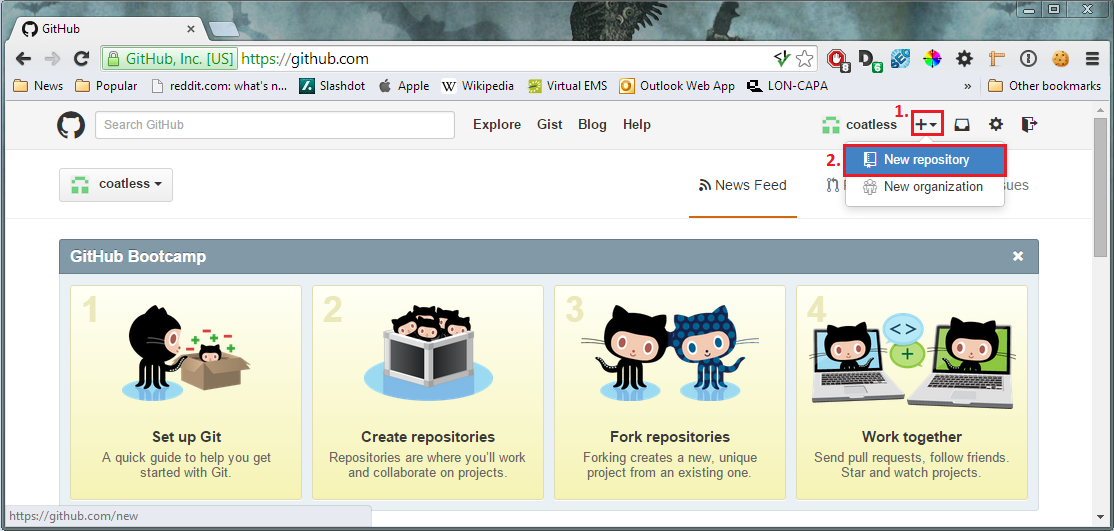
\includegraphics[scale=0.41]{img/git/create_repo.png}
\end{center}

\end{frame}

\begin{frame}
\frametitle{Create a GitHub Repository}
When establishing the repository, consider adding a license to your code.
\begin{center}
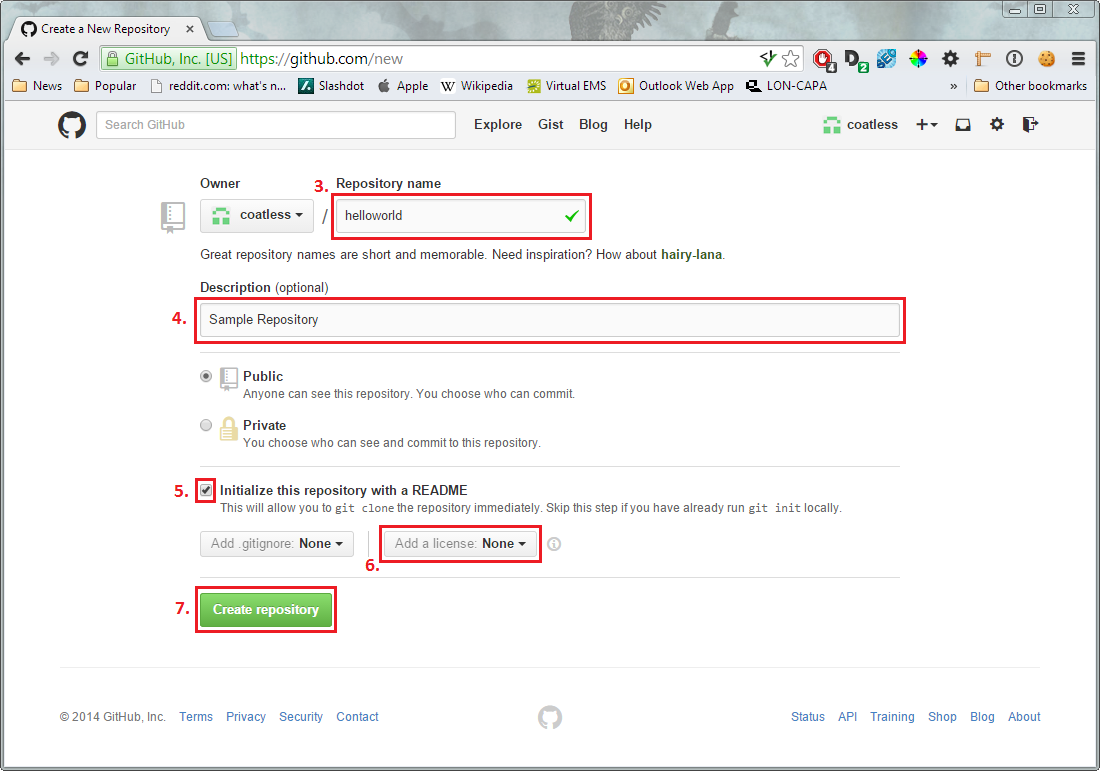
\includegraphics[scale=0.32]{img/git/repo_details.png}
\end{center}

\end{frame}

\begin{frame}
\frametitle{Obtain GitHub Repository Link}

\begin{center}
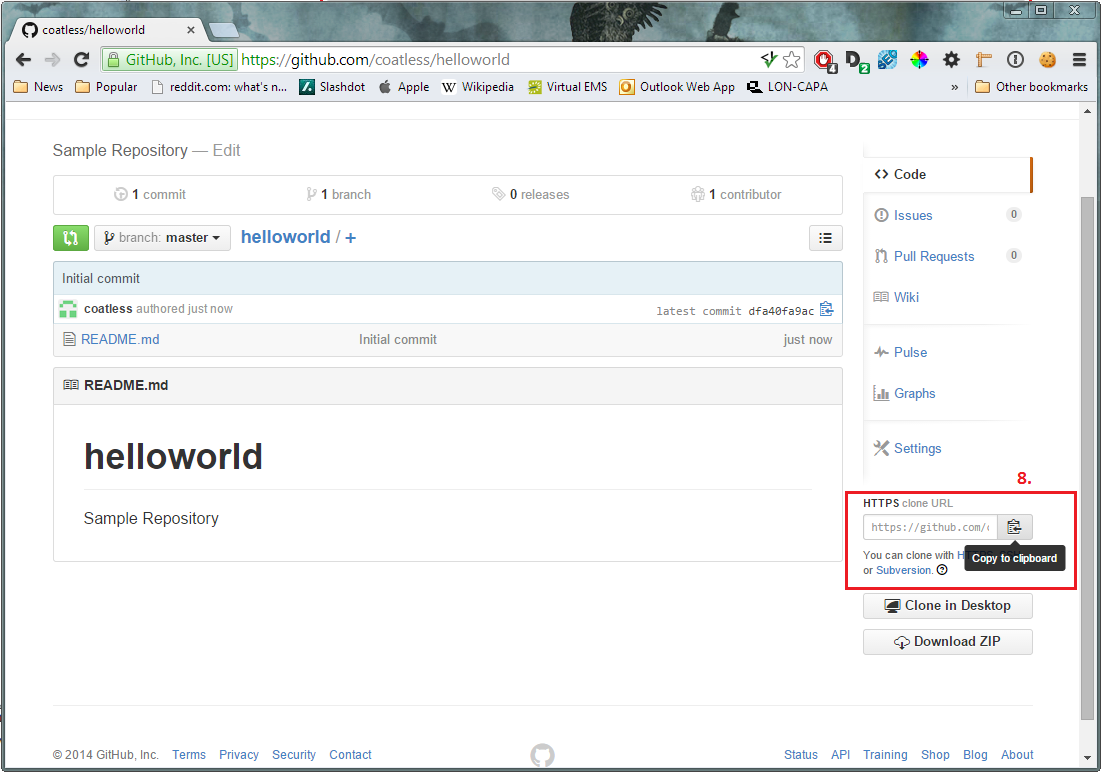
\includegraphics[scale=0.32]{img/git/copy_repository.png}
\end{center}

\end{frame}

\begin{frame}
\frametitle{Create a new R Studio Project}

\begin{columns}[t]
\column{.36\textwidth}
\centering
\begin{block}{Open Project Menu \\ Select `New Project'}
\centering
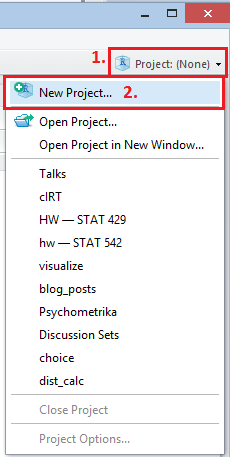
\includegraphics[scale=0.32]{img/project/open_menu.png}
\end{block}
\column{.53\textwidth}
\centering
\begin{block}{Select Version Control}
\centering
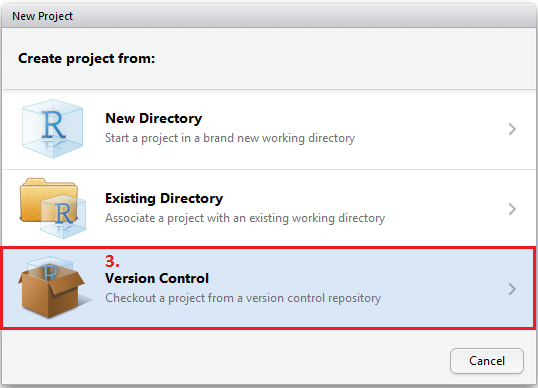
\includegraphics[scale=0.36]{img/project/select_vc_project.png}
\end{block}
\end{columns}
\end{frame}

\begin{frame}
\frametitle{Create a new R Studio Project}

\begin{center}
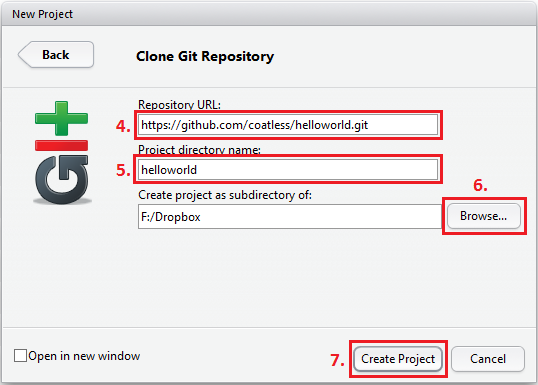
\includegraphics[scale=0.45]{img/project/git_project_details.png}
\end{center}

 
\end{frame}





\begin{frame}
\frametitle{R Studio - Project View}

\begin{center}
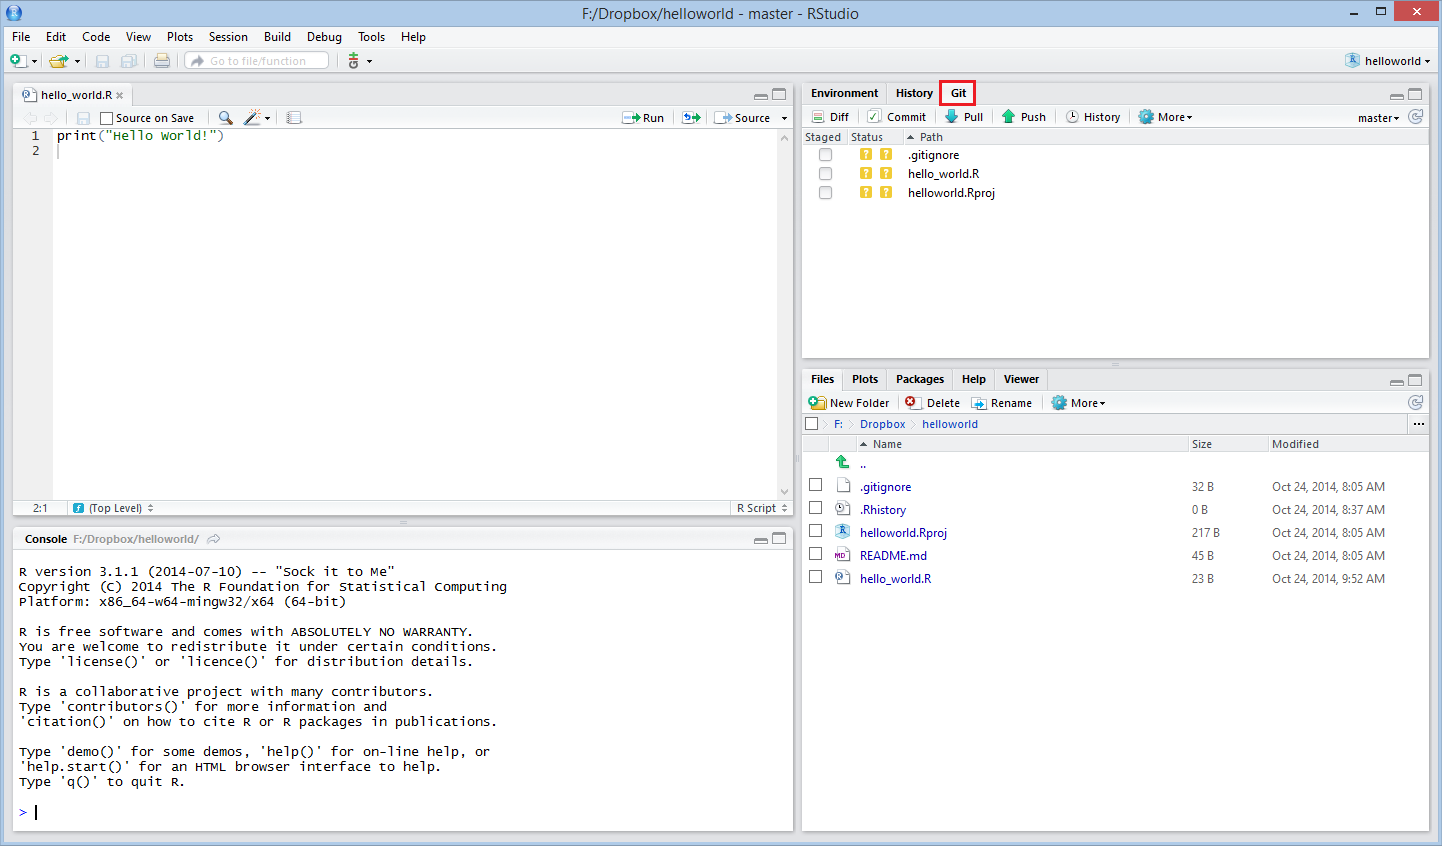
\includegraphics[scale=0.31]{img/project/project_view_git.png}
\end{center}

\end{frame}

\begin{frame}
\frametitle{Using git via R Studio}
\begin{columns}[t]
\column{.45\textwidth}
\centering
\begin{block}{Select file to be staged \\ Press `Commit'}
\centering
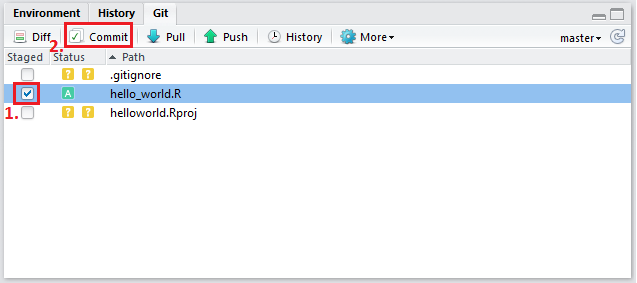
\includegraphics[scale=0.32]{img/project/staging_git.png}
\end{block}
\column{.5\textwidth}
\centering
\begin{block}{Enter commit message \\ Press `Commit' \\ Press `Push'}
\centering
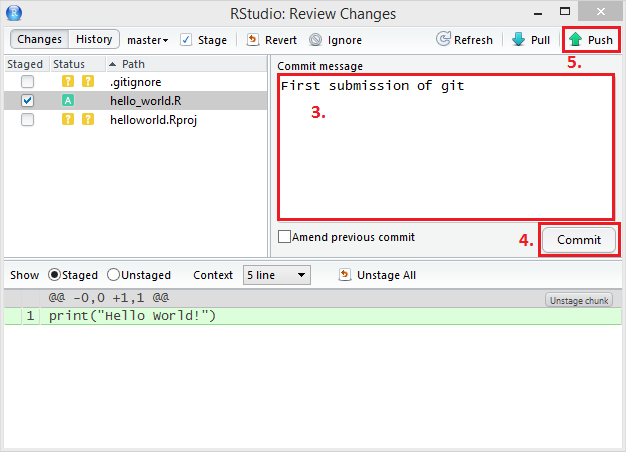
\includegraphics[scale=0.36]{img/project/commit_step_git.png}
\end{block}
\end{columns}

\end{frame}

\begin{frame}
\frametitle{Authorizing...}
One of the downsides of pushing to GitHub is the need to be authenticated...
\begin{center}
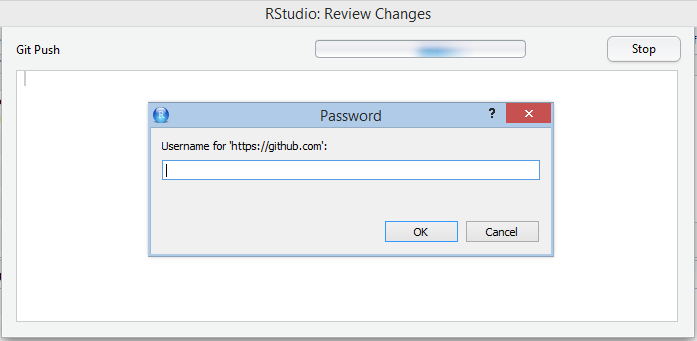
\includegraphics[scale=0.36]{img/project/review_changes.png}
\end{center}

\end{frame}

\begin{frame}[fragile]
\frametitle{Good Authorization via Public and Private SSH Keys}

To simplify this process, we opt to authorize ourselves to GitHub using an encryption technique that uses a \textbf{public and private key scheme}.
\\$ $\\
In this case, the public key is a string of symbols that is out there for the world to see. 
\\$ $\\
On the other hand, the private key is considered to be confidential and only viewable by its owner. 
\\$ $\\
This scheme enables messages signed with the private key to only be viewable via its public key (and vice versa).

\end{frame}



\begin{frame}[fragile]
\frametitle{Good Authorizing - SSH Key Generation}

Instructions for generating an SSH key are given in two flavors:

\begin{enumerate}
\item Using RStudio's GUI
\item Using Shell/Terminal
\end{enumerate}

You only need to pick \textbf{one} route.

\end{frame}

\begin{frame}[fragile]
\frametitle{Good Authorizing - SSH Key Generation via RStudio}

\begin{columns}[t]
\column{.36\textwidth}
\centering
\begin{block}{Click \texttt{`Tools'} \\ Select \texttt{`Global Options'}}
\centering
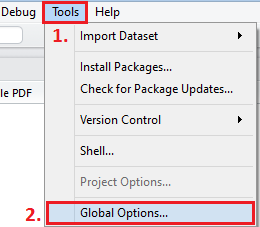
\includegraphics[scale=0.5]{img/configrstudio_opt.png}
\end{block}
\column{.53\textwidth}
\centering
\begin{block}{Click \texttt{`Git/SVN'} \\ Click the \texttt{`Create RSA Key...'}}
\centering
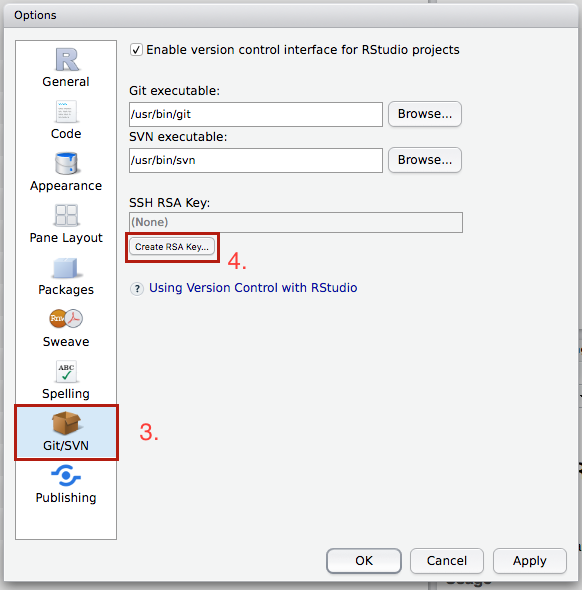
\includegraphics[scale=0.27]{img/ssh/rstudio_blank_ssh.png}
\end{block}
\end{columns}

\end{frame}


\begin{frame}[fragile]
\frametitle{Good Authorizing - SSH Key Generation via RStudio}

\begin{columns}[t]
\column{.36\textwidth}
\centering
\begin{block}{Click \texttt{`Close'}}
\centering
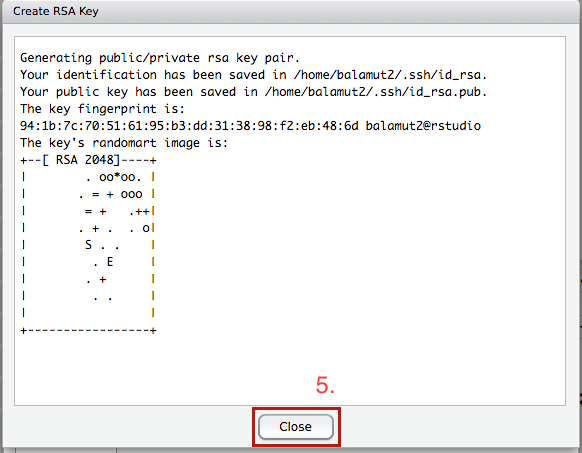
\includegraphics[scale=0.21]{img/ssh/rstudio_succesful_generation.png}
\end{block}
\column{.53\textwidth}
\centering
\begin{block}{Click \texttt{`View Public Key'}}
\centering
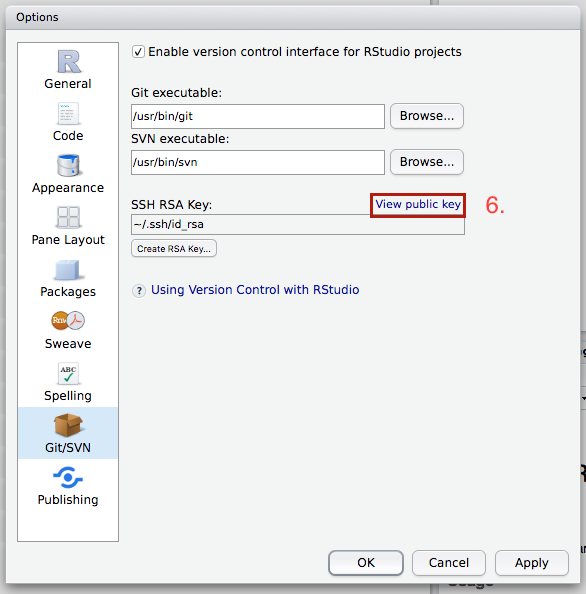
\includegraphics[scale=0.27]{img/ssh/rstudio_ssh_key.png}
\end{block}
\end{columns}

\end{frame}

\begin{frame}[fragile]
\frametitle{Good Authorizing - SSH Key Generation via RStudio}


\begin{block}{Copy the public key with either \\ macOS: \texttt{Command} + \texttt{C} or Windows: \texttt{Cntrl} + \texttt{C}}
\centering
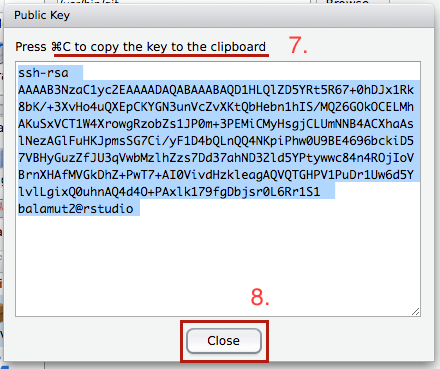
\includegraphics[scale=0.35]{img/ssh/rstudio_public_key.png}
\end{block}

With the key being generated and on our clipboard, we can now add it to our GitHub account... 

\end{frame}

\begin{frame}[fragile]
\frametitle{Good Authorizing - Add Public SSH Key to GitHub}

\begin{columns}[t]
\column{.49\textwidth}
\centering
\begin{block}{Click on the picture in the upper right corner \\ Select \texttt{`Settings'}}
\centering
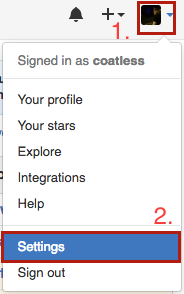
\includegraphics[scale=0.5]{img/ssh/github_settings_menu.png}
\end{block}
\column{.49\textwidth}
\centering
\begin{block}{Click \texttt{`SSH and GPG Keys'}}
\centering
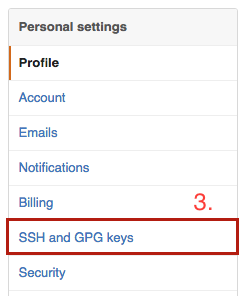
\includegraphics[scale=0.4]{img/ssh/github_profile_menu.png}
\end{block}
\end{columns}

\end{frame}


\begin{frame}[fragile]
\frametitle{Good Authorizing - Add Public SSH Key to GitHub}

\begin{block}{Press the \texttt{`New SSH Key'} button}
\centering
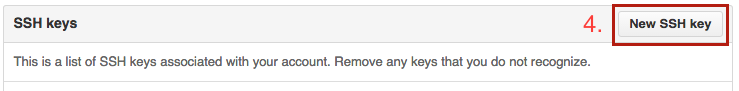
\includegraphics[scale=0.35]{img/ssh/github_new_ssh_key.png}
\end{block}

\begin{block}{Fill in the \texttt{`Title'} input and paste the SSH into \texttt{`Key'} with either \\ macOS: \texttt{Command} + \texttt{V} or Windows: \texttt{Cntrl} + \texttt{V}}
\centering
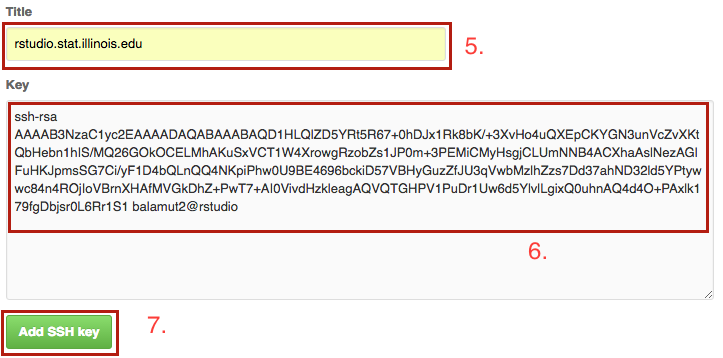
\includegraphics[scale=0.32]{img/ssh/github_ssh_key_add_example.png}
\end{block}

\end{frame}

\begin{frame}[fragile]
\frametitle{Good Authorizing - Add Public SSH Key to GitHub}

\begin{block}{Check that the key has been added}
\centering

\includegraphics[scale=0.45]{img/ssh/github_added_success.png}
\end{block}

If you have made it to this step, well done! 
\\$ $\\$ $\\
\centering
\Large
\textbf{You can now officially commit via SSH.}

\end{frame}


\begin{frame}[fragile]
\frametitle{Good Authorizing - SSH Key Generation}

As promised, next up are the instructions for SSH key generation within Terminal/Shell...
\\$ $\\$ $\\$ $

\Large
\centering
Do \textbf{NOT} repeat this if you opted for the RStudio approach.

\end{frame}

\begin{frame}[fragile]
\frametitle{Good Authorizing - SSH Authorization via Terminal}

Use SSH Authorization by opening terminal/shell (in RStudio access it via Git tab's More $->$ Shell)

\begin{knitrout}\footnotesize
\definecolor{shadecolor}{rgb}{0.969, 0.969, 0.969}\color{fgcolor}\begin{kframe}
\noindent
\ttfamily
\hlstd{ssh{-}keygen\ }\hlopt{{-}}\hlstd{t\ rsa\ }\hlopt{{-}}\hlstd{b\ }\hlnum{4096\ }\hlstd{}\hlopt{{-}}\hlstd{C\ }\hlstr{"your\textunderscore email@example.com"}\hlstd{\ }\hlslc{\#\ Creates\ new\ SSH\ Key}\hspace*{\fill}\\
\hlstd{}\hspace*{\fill}\\
\hlslc{\#\ After\ the\ key\ is\ generated,\ you\ will\ be\ prompted\ with}\hspace*{\fill}\\
\hlstd{Enter\ a\ }\hlkwc{file\ }\hlstd{}\hlkwa{in\ }\hlstd{}\hlkwc{which\ }\hlstd{to\ save\ the\ key\ }\hlopt{(/}\hlstd{Users}\hlopt{/}\hlstd{you}\hlopt{/}\hlstd{.}\hlkwc{ssh}\hlstd{}\hlopt{/}\hlstd{id\textunderscore rsa}\hlopt{):\ {[}}\hlstd{Press\ enter}\hlopt{{]}}\hspace*{\fill}\\
\hlstd{}\hspace*{\fill}\\
\hlslc{\#\ Create\ a\ password\ for\ the\ key\ (needs\ to\ be\ rememberable)}\hspace*{\fill}\\
\hlstd{Enter\ passphrase\ }\hlopt{(}\hlstd{empty\ }\hlkwa{for\ }\hlstd{no\ passphrase}\hlopt{):\ {[}}\hlstd{Type\ a\ passphrase}\hlopt{{]}}\hspace*{\fill}\\
\hlstd{Enter\ same\ passphrase\ again}\hlopt{:\ {[}}\hlstd{Type\ passphrase\ again}\hlopt{{]}}\hspace*{\fill}\\
\hlstd{}\hspace*{\fill}\\
\hlslc{\#\ Start\ the\ SSH\ Agent}\hspace*{\fill}\\
\hlstd{}\hlkwb{eval\ }\hlstd{}\hlstr{"\$(ssh{-}agent\ {-}s)"}\hlstd{}\hspace*{\fill}\\
\hspace*{\fill}\\
\hlslc{\#\ Add\ the\ key}\hspace*{\fill}\\
\hlstd{ssh{-}add\ $\sim$}\hlopt{/}\hlstd{.}\hlkwc{ssh}\hlstd{}\hlopt{/}\hlstd{id\textunderscore rsa}\hspace*{\fill}
\mbox{}
\normalfont
\end{kframe}
\end{knitrout}

\end{frame}

\begin{frame}[fragile]

Copy key to clipboard

Windows:
\begin{knitrout}\footnotesize
\definecolor{shadecolor}{rgb}{0.969, 0.969, 0.969}\color{fgcolor}\begin{kframe}
\noindent
\ttfamily
\hlstd{clip\ }\hlopt{$<$\ }\hlstd{$\sim$}\hlopt{/}\hlstd{.}\hlkwc{ssh}\hlstd{}\hlopt{/}\hlstd{id\textunderscore rsa.pub}\hspace*{\fill}
\mbox{}
\normalfont
\end{kframe}
\end{knitrout}

macOS:
\begin{knitrout}\footnotesize
\definecolor{shadecolor}{rgb}{0.969, 0.969, 0.969}\color{fgcolor}\begin{kframe}
\noindent
\ttfamily
\hlstd{pbcopy\ }\hlopt{$<$\ }\hlstd{$\sim$}\hlopt{/}\hlstd{.}\hlkwc{ssh}\hlstd{}\hlopt{/}\hlstd{id\textunderscore rsa.pub}\hspace*{\fill}
\mbox{}
\normalfont
\end{kframe}
\end{knitrout}

Then we add the key to GitHub using the previous steps... 
\end{frame}

\begin{frame}[fragile]
\frametitle{Bad Authorizing - Use this approach when everything fails}

\begin{center}
\textcolor{red}{This is a very bad option since R Studio does NOT hash .proj files.}
\end{center}

When you enter in your GitHub repository to create your R Project, append your username and password like so to the URL:
\begin{knitrout}
\definecolor{shadecolor}{rgb}{0.969, 0.969, 0.969}\color{fgcolor}\begin{kframe}
\noindent
\ttfamily
\hlstd{https}\hlopt{://}\hlstd{username}\hlopt{:}\hlstd{password@github.com}\hlopt{/}\hlstd{username}\hlopt{/}\hlstd{helloworld.git}\hspace*{\fill}
\mbox{}
\normalfont
\end{kframe}
\end{knitrout}
\end{frame}



\begin{frame}
\frametitle{Using git via shell}

\begin{columns}[t]
\column{.45\textwidth}
\centering
\begin{block}{Select `More' \\ Click `Shell'}
\centering
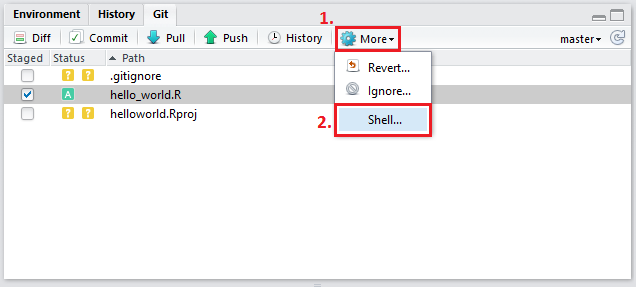
\includegraphics[scale=0.32]{img/project/access_shell_git.png}
\end{block}
\column{.5\textwidth}
\centering
\begin{block}{Type the commands on the next slide}
\centering
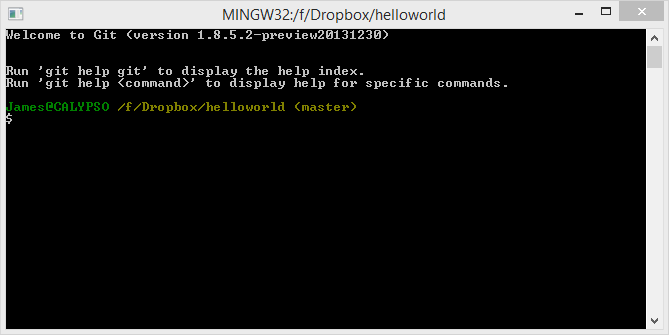
\includegraphics[scale=0.34]{img/git/git_terminal.png}
\end{block}
\end{columns}

\end{frame}

\begin{frame}[fragile]
\frametitle{Using git via shell}
\begin{knitrout}\footnotesize
\definecolor{shadecolor}{rgb}{0.969, 0.969, 0.969}\color{fgcolor}\begin{kframe}
\noindent
\ttfamily
\hlstd{}\hlslc{\#\ Start\ a\ new\ feature}\hspace*{\fill}\\
\hlstd{git\ checkout\ master}\hlstd{\ \ \ \ \ }\hlstd{}\hlslc{\#\ Switch\ to\ master}\hspace*{\fill}\\
\hlstd{git\ branch\ new\textunderscore world}\hlstd{\ \ \ \ }\hlstd{}\hlslc{\#\ Create\ a\ development\ branch}\hspace*{\fill}\\
\hlstd{}\hlslc{\#\ or:\ git\ checkout\ {-}b\ new\textunderscore world\ master}\hspace*{\fill}\\
\hlstd{}\hspace*{\fill}\\
\hlslc{\#\ Add\ a\ new\ file}\hspace*{\fill}\\
\hlstd{git\ add\ hello\textunderscore world.R\hspace*{\fill}\\
git\ commit\ }\hlopt{{-}}\hlstd{m\ }\hlstr{"First\ submission\ of\ git"}\hlstd{}\hspace*{\fill}\\
\hspace*{\fill}\\
\hlslc{\#\ Merge\ in\ the\ new\textunderscore world\ branch}\hspace*{\fill}\\
\hlstd{git\ checkout\ master}\hlstd{\ \ \ \ \ \ }\hlstd{}\hlslc{\#\ Switch\ to\ master}\hspace*{\fill}\\
\hlstd{git\ merge\ new\textunderscore world}\hlstd{\ \ \ \ \ \ }\hlstd{}\hlslc{\#\ Merge\ in\ change}\hspace*{\fill}\\
\hlstd{git\ branch\ }\hlopt{{-}}\hlstd{d\ new\textunderscore world}\hlstd{\ \ }\hlstd{}\hlslc{\#\ Remove\ development\ branch}\hspace*{\fill}\\
\hlstd{}\hspace*{\fill}\\
\hlslc{\#\ Push\ update}\hspace*{\fill}\\
\hlstd{git\ push\ origin\ master}\hspace*{\fill}
\mbox{}
\normalfont
\end{kframe}
\end{knitrout}
\end{frame}

\section{Dynamic Documents}
\subsection{.Rmd documents}

\begin{frame}[fragile]
\frametitle{Markdown}

\href{http://daringfireball.net/projects/markdown/}{\textbf{Markdown}} allows you to write a file format independent document using an easy-to-read and easy-to-write plain text format.
\\$ $\\
In essence, instead of marking up text similar to HTML:
\\
e.g. $<$html$><$body$><$b$>$Name$<$/b$><$/body$><$/html$>$
\\$ $\\
The goal is to mark down text to the simpliest form:
\\
e.g. **Name**
\\$ $\\
As a result of documents being structured so loosely, any file format can really be applied to the rules using \href{http://johnmacfarlane.net/pandoc/}{pandoc}. 
\\$ $\\
\textbf{The downside is that there is less control over formatting.}
\end{frame}

\begin{frame}[fragile]
\frametitle{R Markdown}
\href{http://rmarkdown.rstudio.com/}{R Markdown} developed by \href{http://RStudio.com}{RStudio} takes what Markdown has established and extends it 10x fold.  
\begin{itemize}
\item Merge R code with Markdown
\item Export options quadrupled
\item R Markdown documents are fully reproducible
\item So many more extras vs. the original Markdown
\end{itemize}
\end{frame}

\begin{frame}
\frametitle{Creating a .Rmd Document}
To create a .Rmd Document within R Studio:

\begin{columns}[t]
\column{.32\textwidth}
\centering
\begin{block}{Click the \textcolor{white}{White Plus} \\  Select \texttt{`R Markdown'}}
\centering
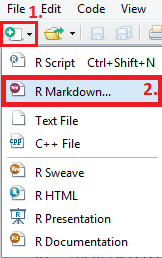
\includegraphics[scale=0.5]{img/rmd/file_new_rmd.png}
\end{block}
\column{.5\textwidth}
\centering
\begin{block}{Enter Document Title}
\centering
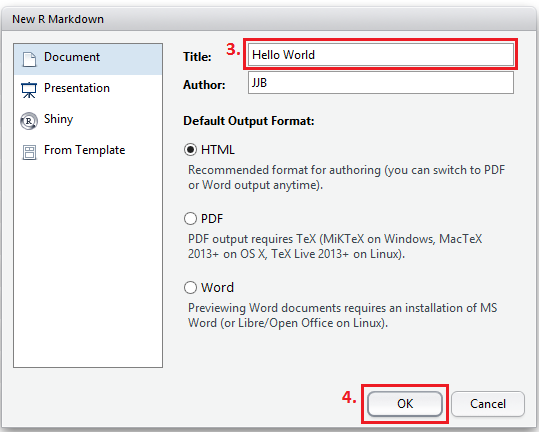
\includegraphics[scale=0.35]{img/rmd/select_new_rmd.png}
\end{block}
\end{columns}
$ $\\
\end{frame}

\begin{frame}
\frametitle{.Rmd View}
\begin{center}
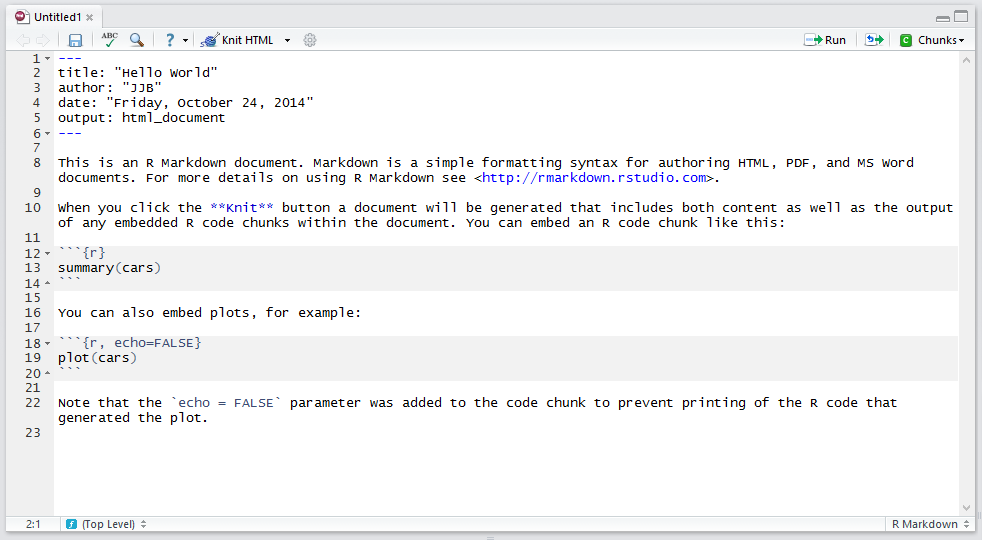
\includegraphics[scale=0.40]{img/rmd/default_rmd.png}
\end{center}
\end{frame}

\begin{frame}
\frametitle{Text Features of RMarkdown}
\begin{center}
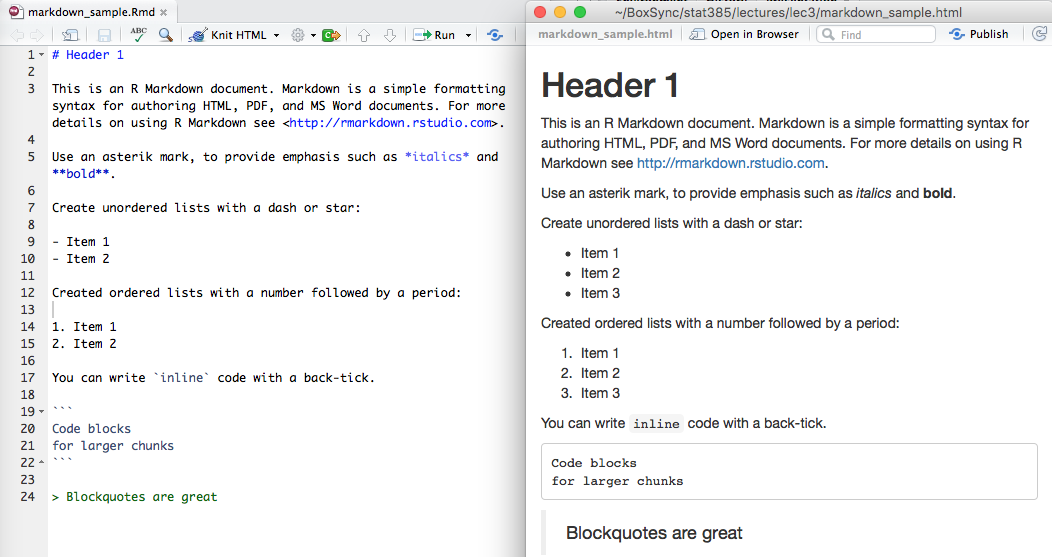
\includegraphics[scale=.3]{img/rmd/rmarkdown_overview.png}
\end{center}
\end{frame}

\begin{frame}[fragile]
\frametitle{Code Chunks, this time for .Rmd}
To initiate a code chunk within .Rmd, all one needs to do is use:
\begin{knitrout}
\definecolor{shadecolor}{rgb}{0.969, 0.969, 0.969}\color{fgcolor}\begin{kframe}
\begin{alltt}
```\{r chunk_label\}
\hlcom{# Code here}
```
\end{alltt}
\end{kframe}
\end{knitrout}
Example:
\begin{knitrout}
\definecolor{shadecolor}{rgb}{0.969, 0.969, 0.969}\color{fgcolor}\begin{kframe}
\begin{alltt}
Here is a sample way of usings chunk options
```\{r chunk_label, eval=FALSE\}
opts_chunk$\hlkwd{set}(warning=FALSE, message=FALSE)
\hlkwd{set.seed}(1337)
```
More text...
\end{alltt}
\end{kframe}
\end{knitrout}

\textbf{Chunk options are the same between .Rnw and .Rmd}
\end{frame}

\begin{frame}[fragile]
\frametitle{In-line R code for .Rmd}

.Rmd has the ability to write inline using: `r expression\textunderscore here`
\\$ $\\
Example:
\begin{knitrout}
\definecolor{shadecolor}{rgb}{0.969, 0.969, 0.969}\color{fgcolor}\begin{kframe}
\begin{alltt}
Did you know that there are `r \hlkwd{dim}(apples)[1]` observations 
and `r \hlkwd{dim}(apples)[2]` variables contained within the apples 
data set?
\end{alltt}
\end{kframe}
\end{knitrout}
Note:
\begin{itemize}
\item All inline commands must be on the same line (no returns)!
\item Helpful to have code chunk hidden before paragraph and use inline features to control output.
\end{itemize}

\end{frame}

\begin{frame}[fragile]
\frametitle{Output options}
The key to .Rmd's strength is in the output statement  at the front of the document.
There are so many options to customize the final output. 
\begin{knitrout}
\definecolor{shadecolor}{rgb}{0.969, 0.969, 0.969}\color{fgcolor}\begin{kframe}
\noindent
\ttfamily
\hlstd{}\hlopt{{-}{-}{-}}\hspace*{\fill}\\
\hlstd{title}\hlopt{:\ }\hlstd{}\hlstr{"Sample\ Document"}\hlstd{\hspace*{\fill}\\
author}\hlopt{:\ }\hlstd{}\hlstr{"James\ Balamuta"}\hlstd{}\hspace*{\fill}\\
\hlkwc{date}\hlstd{}\hlopt{:\ }\hlstd{}\hlstr{"June\ 16,\ 2016"}\hlstd{\hspace*{\fill}\\
output}\hlopt{:}\hspace*{\fill}\\
\hlstd{}\hlstd{\ \ }\hlstd{pdf\textunderscore document}\hlopt{:}\hspace*{\fill}\\
\hlstd{}\hlstd{\ \ \ \ }\hlstd{toc}\hlopt{:\ }\hlstd{true}\hlstd{\ \ \ \ \ \ \ \ \ \ \ \ \ }\hlstd{}\hlslc{\#\ Table\ of\ Contents}\hspace*{\fill}\\
\hlstd{}\hlstd{\ \ \ \ }\hlstd{toc\textunderscore depth}\hlopt{:\ }\hlstd{}\hlnum{2}\hlstd{\ \ \ \ \ \ \ \ \ \ }\hlnum{}\hlstd{}\hlslc{\#\ Nested\ 2\ levels}\hspace*{\fill}\\
\hlstd{}\hlstd{\ \ \ \ }\hlstd{number\textunderscore sections}\hlopt{:\ }\hlstd{true\ }\hlslc{\#\ Number\ Sections}\hspace*{\fill}\\
\hlstd{}\hlstd{\ \ \ \ }\hlstd{highlight}\hlopt{:\ }\hlstd{}\hlstr{"zenburn"}\hlstd{}\hlstd{\ \ }\hlstd{}\hlslc{\#\ Code\ Highlighting}\hspace*{\fill}\\
\hlstd{}\hlstd{\ \ \ \ }\hlstd{keep\textunderscore tex}\hlopt{:\ }\hlstd{true}\hlstd{\ \ \ \ \ \ \ \ }\hlstd{}\hlslc{\#\ Retain\ .tex\ file\ used\ for\ .pdf}\hspace*{\fill}\\
\hlstd{}\hlopt{{-}{-}{-}}\hlstd{}\hspace*{\fill}
\mbox{}
\normalfont
\end{kframe}
\end{knitrout}
\end{frame}

\begin{frame}[fragile]
\frametitle{Outputing multiple files from a single .Rmd}
\begin{knitrout}
\definecolor{shadecolor}{rgb}{0.969, 0.969, 0.969}\color{fgcolor}\begin{kframe}
\noindent
\ttfamily
\hlstd{}\hlopt{{-}{-}{-}}\hspace*{\fill}\\
\hlstd{title}\hlopt{:\ }\hlstd{}\hlstr{"Sample\ Document"}\hlstd{\hspace*{\fill}\\
author}\hlopt{:\ }\hlstd{}\hlstr{"James\ Balamuta"}\hlstd{\hspace*{\fill}\\
output}\hlopt{:}\hspace*{\fill}\\
\hlstd{}\hlstd{\ \ }\hlstd{html\textunderscore document}\hlopt{:}\hspace*{\fill}\\
\hlstd{}\hlstd{\ \ \ \ }\hlstd{toc}\hlopt{:\ }\hlstd{true}\hlstd{\ \ \ \ \ \ \ \ \ \ \ \ }\hlstd{}\hlslc{\#\ Table\ of\ contents}\hspace*{\fill}\\
\hlstd{}\hlstd{\ \ \ \ }\hlstd{theme}\hlopt{:\ }\hlstd{cerulean}\hlstd{\ \ \ \ \ \ }\hlstd{}\hlslc{\#\ Bootstrap\ theme}\hspace*{\fill}\\
\hlstd{}\hlstd{\ \ }\hlstd{pdf\textunderscore document}\hlopt{:}\hspace*{\fill}\\
\hlstd{}\hlstd{\ \ \ \ }\hlstd{toc}\hlopt{:\ }\hlstd{true}\hlstd{\ \ \ \ \ \ \ \ \ \ \ \ }\hlstd{}\hlslc{\#\ Table\ of\ contents}\hspace*{\fill}\\
\hlstd{}\hlstd{\ \ \ \ }\hlstd{keep\textunderscore tex}\hlopt{:\ }\hlstd{true}\hlstd{\ \ \ \ \ \ \ }\hlstd{}\hlslc{\#\ Retain\ .tex\ file\ used\ for\ .pdf}\hspace*{\fill}\\
\hlstd{}\hlstd{\ \ }\hlstd{word\textunderscore document}\hlopt{:}\hspace*{\fill}\\
\hlstd{}\hlstd{\ \ \ \ }\hlstd{fig\textunderscore width}\hlopt{:\ }\hlstd{}\hlnum{5}\hlstd{\ \ \ \ \ \ \ \ \ }\hlnum{}\hlstd{}\hlslc{\#\ Set\ figure\ width}\hspace*{\fill}\\
\hlstd{}\hlstd{\ \ \ \ }\hlstd{fig\textunderscore height}\hlopt{:\ }\hlstd{}\hlnum{5}\hlstd{\ \ \ \ \ \ \ \ }\hlnum{}\hlstd{}\hlslc{\#\ Set\ figure\ height}\hspace*{\fill}\\
\hlstd{}\hlstd{\ \ \ \ }\hlstd{fig\textunderscore caption}\hlopt{:\ }\hlstd{true}\hlstd{\ \ \ \ }\hlstd{}\hlslc{\#\ Output\ captions\ with\ figures}\hspace*{\fill}\\
\hlstd{}\hlopt{{-}{-}{-}}\hlstd{}\hspace*{\fill}
\mbox{}
\normalfont
\end{kframe}
\end{knitrout}
\end{frame}

\begin{frame}[fragile]
\frametitle{Compiling .Rmd to .*}
Compile via R Studio to .html document:

\includegraphics[scale=0.5]{img/rmd/compile_rmd.png}
\\$ $\\
Switching to a different output format (pdf in this case): \\
\begin{center}

\includegraphics[scale=0.5]{img/rmd/other_options.png}
\end{center}
\end{frame}

\begin{frame}[fragile]
\frametitle{Compiling .Rmd to .* }
Compile .Rmd via r console...
\\$ $\\
Single line output declarations
\begin{knitrout}
\definecolor{shadecolor}{rgb}{0.969, 0.969, 0.969}\color{fgcolor}\begin{kframe}
\begin{alltt}
\hlkwd{library}\hlstd{(knitr)}
\hlkwd{knit2html}\hlstd{(}\hlstr{'input.Rmd'}\hlstd{)} \hlcom{# Creates .html file}
\hlkwd{knit2pdf}\hlstd{(}\hlstr{'input.Rmd'}\hlstd{)}  \hlcom{# Creates .pdf file}
\hlkwd{knit}\hlstd{(}\hlstr{'input.Rmd'}\hlstd{)}      \hlcom{# Creates .md file}
\end{alltt}
\end{kframe}
\end{knitrout}

Or use for multiline output declarations
\begin{knitrout}
\definecolor{shadecolor}{rgb}{0.969, 0.969, 0.969}\color{fgcolor}\begin{kframe}
\begin{alltt}
\hlkwd{library}\hlstd{(rmarkdown)}
\hlkwd{render}\hlstd{(}\hlstr{"input.Rmd"}\hlstd{,} \hlstr{"pdf_document"}\hlstd{)}
\hlkwd{render}\hlstd{(}\hlstr{"input.Rmd"}\hlstd{,} \hlstr{"word_document"}\hlstd{)}
\hlkwd{render}\hlstd{(}\hlstr{"input.Rmd"}\hlstd{,} \hlstr{"md_document"}\hlstd{)}
\end{alltt}
\end{kframe}
\end{knitrout}
\end{frame}

\begin{frame}
\frametitle{Options... Options... Options...}
Some of .Rmd's output options can be configured via a GUI in R Studio:
\begin{center}

\includegraphics[scale=0.5]{img/rmd/rmd_options.png}
\end{center}
\begin{center}
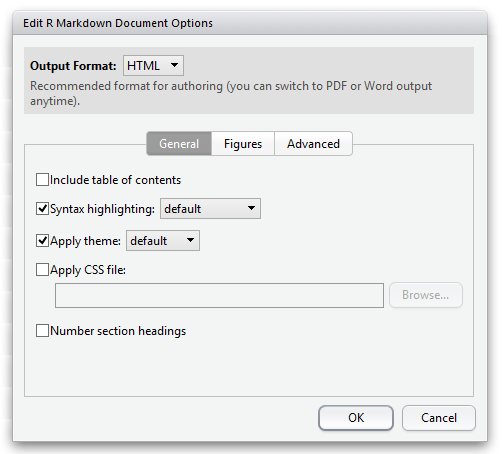
\includegraphics[scale=0.35]{img/rmd/rmd_options_in_rstudio.png}
\end{center}

To see all the options granted by .Rmd, check out the package website at:
\url{http://rmarkdown.rstudio.com/}. 
\end{frame}


\begin{frame}[fragile]
\frametitle{Fun Application of .Rmd}
Create a new blog post on a Wordpress site using R:
\begin{knitrout}\tiny
\definecolor{shadecolor}{rgb}{0.969, 0.969, 0.969}\color{fgcolor}\begin{kframe}
\begin{alltt}
\hlcom{# Check to see if RWordPress is install and install if necessary.}
\hlkwa{if} \hlstd{(}\hlopt{!}\hlkwd{require}\hlstd{(}\hlstr{'RWordPress'}\hlstd{))}
  \hlkwd{install.packages}\hlstd{(}\hlstr{'RWordPress'}\hlstd{,} \hlkwc{repos} \hlstd{=} \hlstr{'http://www.omegahat.org/R'}\hlstd{,} \hlkwc{type} \hlstd{=} \hlstr{'source'}\hlstd{)}

\hlcom{# Load Library}
\hlkwd{library}\hlstd{(RWordPress)}
\hlcom{# Pass user credentials}
\hlkwd{options}\hlstd{(}\hlkwc{WordpressLogin} \hlstd{=} \hlkwd{c}\hlstd{(}\hlkwc{Username} \hlstd{=} \hlstr{'password'}\hlstd{),}
        \hlkwc{WordpressURL} \hlstd{=} \hlstr{'http://publish.illinois.edu/<netid>/xmlrpc.php'}\hlstd{)}

\hlcom{# Initialize knitr}
\hlkwd{library}\hlstd{(knitr)}

\hlcom{# Uploads r generated images to server. Can be switched to imgur, etc.}
\hlstd{opts_knit}\hlopt{$}\hlkwd{set}\hlstd{(}\hlkwc{upload.fun} \hlstd{=} \hlkwa{function}\hlstd{(}\hlkwc{file}\hlstd{)\{}
  \hlkwd{library}\hlstd{(RWordPress)}
  \hlkwd{uploadFile}\hlstd{(file)}\hlopt{$}\hlstd{url}
\hlstd{\})}

\hlcom{# Push rmarkdown to wordpress site}
\hlkwd{knit2wp}\hlstd{(}\hlstr{'file_name.Rmd'}\hlstd{,} \hlkwc{title} \hlstd{=} \hlstr{'Test r post'}\hlstd{)}
\end{alltt}
\end{kframe}
\end{knitrout}
\end{frame}

\subsection{Features of \texttt{knitr}}

\begin{frame}[fragile]
\frametitle{Setting Global Chunk Options}
Instead of declaring options repetitively across multiple code chunks, it is better to create a global declaration in a ``setup" chunk at the start of the document. 
\\$ $\\
Even with a global declaration, values are able to be changed locally on code chunks on an as needed basis. The local values will not affect future code chunks.
\\$ $\\
To set global chunk settings use:
\begin{knitrout}
\definecolor{shadecolor}{rgb}{0.969, 0.969, 0.969}\color{fgcolor}\begin{kframe}
\begin{alltt}
```\{r set_global\}
opts_chunk$\hlkwd{set}(eval = FALSE, comment=NA, 
               fig.width=6, fig.height=6, 
               fig.align=\hlstr{'center'})
```
\end{alltt}
\end{kframe}
\end{knitrout}
\end{frame}

\begin{frame}[fragile]
\frametitle{Caching}
\textbf{Caching} refers to storing data locally in order to speed up subsequent retrievals.
\\$ $\\
In essence, the code chunk will be run once, the resulting objects are then stored within a file, and the stored data is then displayed on subsequent runs.
\\$ $\\
This feature is very handy when embedding analysis on large data sets or time intensive computations.
\end{frame}

\begin{frame}[fragile]
\frametitle{Be Careful When Caching...}
Simple yet problematic cache:
\begin{knitrout}
\definecolor{shadecolor}{rgb}{0.969, 0.969, 0.969}\color{fgcolor}\begin{kframe}
\begin{alltt}
```\{r cache_demo, cache = T\}
x = \hlkwd{rnorm}(5)
```
\end{alltt}
\end{kframe}
\end{knitrout}
\begin{knitrout}
\definecolor{shadecolor}{rgb}{0.969, 0.969, 0.969}\color{fgcolor}\begin{kframe}
\begin{verbatim}
## [1] -0.3407 -0.3130 -0.2468  0.4668  0.5254
\end{verbatim}
\end{kframe}
\end{knitrout}
\end{frame}


\begin{frame}[fragile]
\frametitle{The Problematic Cache}
Suppose you have three chunks, $A$, $B$, and $C$, that have RNG and have been cached.
\\$ $\\
If chunk $C$ is inserted between $A$ and $B$, then $B$ should be updated because RNG modifies .Random.seed as a side-effect, but the chunk $B$ will \textit{not} be updated
\\$ $\\
$\Rightarrow$ The reproducibility of $B$ is bogus.
\\$ $\\
To guarantee reproducibility with RNG, .Random.seed needs to be associated with the cache for each chunk using:
\begin{knitrout}
\definecolor{shadecolor}{rgb}{0.969, 0.969, 0.969}\color{fgcolor}\begin{kframe}
\begin{alltt}
\hlcom{# Set global chunk options}
\hlstd{opts_chunk}\hlopt{$}\hlkwd{set}\hlstd{(}\hlkwc{cache.extra} \hlstd{= rand_seed)}
\end{alltt}
\end{kframe}
\end{knitrout}
\end{frame}

\begin{frame}[fragile]
\frametitle{The Limiting Cache Scope}
Sometimes the cache needs to be limited by R version, Session Info, or a time stamp.
\begin{knitrout}
\definecolor{shadecolor}{rgb}{0.969, 0.969, 0.969}\color{fgcolor}\begin{kframe}
\begin{alltt}
\hlcom{# Set global chunk options}
opts_chunk$\hlkwd{set}(cache.extra = 
                 \hlkwd{list}(R.version,     \hlcom{# R version info w/ OS}
                      rand_seed,     \hlcom{# .Random.seed}
                      \hlkwd{sessionInfo}(), \hlcom{# Current Configuration}
\hlcom{                      # Month timestamp}
                      \hlkwd{format}(\hlkwd{Sys.Date}(), \hlstr{'%Y-%m'})) 
\end{alltt}
\end{kframe}
\end{knitrout}
\end{frame}

\begin{frame}[fragile]
\frametitle{Limit Cache by File Info}

Limit cache using the file stamp associated with data files being read into R for the analysis
\begin{knitrout}
\definecolor{shadecolor}{rgb}{0.969, 0.969, 0.969}\color{fgcolor}\begin{kframe}
\begin{alltt}
\hlcom{#' @param files is a character vector containing filenames}
\hlcom{#' @return time stamp}
\hlstd{mtime} \hlkwb{=} \hlkwa{function}\hlstd{(}\hlkwc{files}\hlstd{)\{}
  \hlkwd{lapply}\hlstd{(}\hlkwd{Sys.glob}\hlstd{(files),}\hlkwa{function}\hlstd{(}\hlkwc{x}\hlstd{)} \hlkwd{file.info}\hlstd{(x)}\hlopt{$}\hlstd{mtime)}
\hlstd{\}}
\end{alltt}
\end{kframe}
\end{knitrout}

\begin{knitrout}
\definecolor{shadecolor}{rgb}{0.969, 0.969, 0.969}\color{fgcolor}\begin{kframe}
\begin{alltt}
```\{r data_read_in, cache.extra=\hlkwd{mtime}(\hlstr{"apple.csv"})\}
```
\end{alltt}
\end{kframe}
\end{knitrout}
\end{frame}


\begin{frame}[fragile]
\frametitle{Returning to In-line R code for .Rmd}

Previously, we executed code inline with an actual function call: 
\begin{knitrout}
\definecolor{shadecolor}{rgb}{0.969, 0.969, 0.969}\color{fgcolor}\begin{kframe}
\begin{alltt}
\hlstd{`r dim(apples)[1]`}
\end{alltt}
\end{kframe}
\end{knitrout}
In this case, it is highly preferred to move those calls to a code chunk \emph{before} the text as this calculation can then be cached.
\\$ $\\
Code Chunk Example:
\begin{knitrout}
\definecolor{shadecolor}{rgb}{0.969, 0.969, 0.969}\color{fgcolor}\begin{kframe}
\begin{alltt}
```\{r data_inline_calc, cache = TRUE\}
\hlkwd{data}(\hlstr{"apples"})      # Loads the apple data set.
obs  = \hlkwd{nrow}(apples) \hlcom{# Number of observations in the dataset}
vars = \hlkwd{ncol}(apples) \hlcom{# Number of variables in the dataset}
```
\end{alltt}
\end{kframe}
\end{knitrout}

\end{frame}

\begin{frame}[fragile]
\frametitle{}

In document:
\begin{knitrout}
\definecolor{shadecolor}{rgb}{0.969, 0.969, 0.969}\color{fgcolor}\begin{kframe}
\begin{alltt}
Did you know that there are `r obs` observations 
and `r vars` variables contained within the apples 
data set?
\end{alltt}
\end{kframe}
\end{knitrout}

Compared to the previous approach, we now have:

\begin{itemize}
\item Cached computations
\item Clearer function calls
\item Less obtrusive explanations. 
\end{itemize}

\end{frame}

\begin{frame}[fragile]
\frametitle{Code Externalization}
When we first began using \texttt{knitr}, the R code was directly embedded into the .Rmd file. 
\begin{center}
{\textbf{This is not a good practice in general.} }
\end{center}
Why? The elements of the analysis are then merged with elements of the presentation.
\\$ $\\
If the code is externalized:
\begin{enumerate}
\item The code can be run without compiling the document. 
\item Sharing the code with others is easier.
\item Switch between presentation slides and the code during the actual presentation.
\end{enumerate}
\end{frame}

\begin{frame}[fragile]
\frametitle{Code Externalization in Action}
To externalize code, the r code file must contain comments of the form:
\begin{center}\#\# -\,-\,-\,- label or \#\# @knitr label\end{center}, where label denotes a code chunk name.
\\$ $\\
Example Code File: analysis\_code.R
\begin{knitrout}
\definecolor{shadecolor}{rgb}{0.969, 0.969, 0.969}\color{fgcolor}\begin{kframe}
\begin{alltt}
\hlcom{# Label code as:}

\hlcom{## @knitr external_code}
\hlstd{(x} \hlkwb{=} \hlstr{"Rawr?"}\hlstd{)}

\hlcom{# or }

\hlcom{## ---- external_code}
\hlstd{(x} \hlkwb{=} \hlstr{"Rawr?"}\hlstd{)}
\end{alltt}
\end{kframe}
\end{knitrout}
\end{frame}

\begin{frame}[fragile]
Example .Rmd File: analysis\_writeup.Rmd
\begin{knitrout}
\definecolor{shadecolor}{rgb}{0.969, 0.969, 0.969}\color{fgcolor}\begin{kframe}
\begin{alltt}
```\{r external_code_load, echo=TRUE\}
\hlkwd{read_chunk}(\hlstr{'analysis_code.R'}) \hlcom{# Reads in file, parses comment}
```
\end{alltt}
\end{kframe}
\end{knitrout}

Activate Code Chunk in Document:
\begin{knitrout}
\definecolor{shadecolor}{rgb}{0.969, 0.969, 0.969}\color{fgcolor}\begin{kframe}
\begin{alltt}
```\{r external_code, echo=TRUE\}
```
\end{alltt}
\end{kframe}
\end{knitrout}

Result:
\begin{knitrout}
\definecolor{shadecolor}{rgb}{0.969, 0.969, 0.969}\color{fgcolor}\begin{kframe}
\begin{alltt}
\hlstd{(x} \hlkwb{=} \hlstr{"Rawr?"}\hlstd{)}
\end{alltt}
\begin{verbatim}
## [1] "Rawr?"
\end{verbatim}
\end{kframe}
\end{knitrout}
\end{frame}

\begin{frame}
\frametitle{Reusing Code Chunks}
By labeling code chunks, \texttt{knitr} is able to call them in the future or embed them within other code chunks.
\\$ $\\
To reuse the code from $<<$chunk-name$>>$, call it from within \texttt{```}\{r chunk-embedded\}.
\end{frame}

\begin{frame}[fragile]
\frametitle{Reusing Code Chunks Example}
Initial chunk:
\begin{knitrout}\footnotesize
\definecolor{shadecolor}{rgb}{0.969, 0.969, 0.969}\color{fgcolor}\begin{kframe}
\begin{alltt}
```\{r chunk-name\}
test = \hlstr{"hello"}
```
\end{alltt}
\end{kframe}
\end{knitrout}

Embedded Chunk:
\begin{knitrout}\footnotesize
\definecolor{shadecolor}{rgb}{0.969, 0.969, 0.969}\color{fgcolor}\begin{kframe}
\begin{verbatim}
```{r chunk-embedded}
<<chunk-name>>
```
\end{verbatim}
\end{kframe}
\end{knitrout}

Result:
\begin{knitrout}\footnotesize
\definecolor{shadecolor}{rgb}{0.969, 0.969, 0.969}\color{fgcolor}\begin{kframe}
\begin{alltt}
\hlstr{"hello"}
\end{alltt}
\begin{verbatim}
## [1] "hello"
\end{verbatim}
\end{kframe}
\end{knitrout}
\end{frame}


\begin{frame}[fragile]
\frametitle{Linking to Content}
To link content for Rmd files:
\begin{knitrout}
\definecolor{shadecolor}{rgb}{0.969, 0.969, 0.969}\color{fgcolor}\begin{kframe}
\begin{alltt}
\hlcom{# Only the link}
<http://stat385.thecoatlessprofessor.com>
  
\hlcom{# Create a link for specific text}
[stat385 course material](http://stat385.thecoatlessprofessor.com) 
\end{alltt}
\end{kframe}
\end{knitrout}
\end{frame}

\begin{frame}[fragile]
\frametitle{Including Graphics}
The inclusion of graphics generated outside of R follows a similar scheme as linking to external websites:
\begin{knitrout}
\definecolor{shadecolor}{rgb}{0.969, 0.969, 0.969}\color{fgcolor}\begin{kframe}
\begin{alltt}
\hlcom{# On the Web}
![alt text](http://example.com/logo.png) 

\hlcom{# Locally via relative path}
![alt text](figures/img.png)             
\end{alltt}
\end{kframe}
\end{knitrout}
\end{frame}


\subsection{Dynamic Generation}
\begin{frame}[fragile]
\frametitle{BibTex}
In R Studio, we are able to use BibTex to generate bibliographies.

BibTex is a way to structure output of paper citations you can obtain from \href{https://scholar.google.com/}{Google Scholar}
\\$ $\\
\textbf{Note:} The biber backend for .bib files is not easily supported in R Studio.
\end{frame}

\begin{frame}[fragile]
\frametitle{Structuring a .bib file}
Bibliography information is stored in .bib files. \\
Here is the mybiblib.bib used in the previous example:
\footnotesize
\begin{verbatim}
@article{tv1981,
  title={The framing of decisions and the psychology of choice},
  author={Tversky, Amos and Kahneman, Daniel},
  journal={Science},
  volume={211},
  number={4481},
  pages={453--458},
  year={1981},
  publisher={American Association for the Advancement of Science}
}
@book{ho1987,
  title={Rational choice: Contrast between economics and psychology.},
  author={Hogarth, Robin M and Reder, Melvin W},
  year={1987},
  publisher={University of Chicago Press}
}
\end{verbatim}

\end{frame}

\begin{frame}[fragile]
\frametitle{}

\begin{knitrout}
\definecolor{shadecolor}{rgb}{0.969, 0.969, 0.969}\color{fgcolor}\begin{kframe}
\begin{alltt}
---
title: \hlstr{"Example Biblography heading"}
output: html_document
bibliography: bibliography.bib
---
\end{alltt}
\end{kframe}
\end{knitrout}

Reference in the document using: 

\begin{itemize}
\item Authors + Year
\begin{itemize}
\item "Choice is important" [@ho1987].
\end{itemize}
\item Suppress author information and only have a year
\begin{itemize}
\item Hogarth says, "Choice is important" [-@ho1987].
\end{itemize}
\end{itemize}

\end{frame}



\begin{frame}[fragile]
\frametitle{knitr's \texttt{kable()}}
The main benefit to \texttt{kable()} is not having to worry about the mode \texttt{knitr} is currently in (e.g. html, latex, or markdown) and its ability to split tables over pages.
\\$ $\\ 
Make sure to set the chunk option \texttt{results = `asis'}.
\end{frame}

\begin{frame}[fragile]
\frametitle{Demo of \texttt{kable()}}

\begin{knitrout}
\definecolor{shadecolor}{rgb}{0.969, 0.969, 0.969}\color{fgcolor}\begin{kframe}
\begin{alltt}
```\{r results=\hlstr{'asis'}\}
\hlkwd{kable}(\hlkwd{head}(iris,3),   \hlcom{# Data to be converted to table}
      row.names=TRUE, \hlcom{# Show rownames}
      align=\hlkwd{c}(\hlstr{'l'}, \hlstr{'c'}, \hlstr{'r'}, \hlstr{'l'}, \hlstr{'r'}), \hlcom{# Sets column alignment}
      digits=1        \hlcom{# Restrict amount of digits after decimal}
      )
```
\end{alltt}
\end{kframe}
\end{knitrout}


\begin{tabular}{l|l|c|r|l|r}
\hline
  & Sepal.Length & Sepal.Width & Petal.Length & Petal.Width & Species\\
\hline
1 & 5.1 & 3.5 & 1.4 & 0.2 & setosa\\
\hline
2 & 4.9 & 3.0 & 1.4 & 0.2 & setosa\\
\hline
3 & 4.7 & 3.2 & 1.3 & 0.2 & setosa\\
\hline
\end{tabular}


\end{frame}


\section{Extra}
\subsection{Explanation of Git Commands}

\begin{frame}
\frametitle{Git Commands}
Basic Git Commands:
\begin{description}[labelsep=1in, labelindent=.5cm]
\item[git init:] Initializes a new git repository. (Must be run to setup repo, no repo = no commands working)
\item[git config $<$option$>$:] Configure git options 
\item[git help $<$command$>$:] Provides information on how to use and configure a specific git command.
\item[git status:] See what files are in the repository, what changes need to be committed, and what branch of the repository is active.
\end{description}
\end{frame}

\begin{frame}
\frametitle{Git Commands}
Feature Development Commands:
\begin{description}[labelsep=1in, labelindent=.5cm]
\item[git add $<$file$>$:] Add a new or changed file or files (.) into a ``staging" area.
\item[git commit -m ``Message here" :] Pushes change into the repository with message
\item[git checkout:] A way to select which line of development you're working on. (e.g. Master or your own branch)
\item[git branch $<$name$>$:] Build a new branch off of the active repository to make changes and file additions that are completely your own.
\item[git merge:] Merge changes in your branch back to the master branch.
\end{description}
\end{frame}

\begin{frame}
\frametitle{Git Commands}
Syncing Git Commands:
\begin{description}[labelsep=1in, labelindent=.5cm]
\item[git remote:] Create, view, and delete connections to other repositories. 
\item[git fetch:] Imports commits from a remote repository into your local repository. Helpful for reviewing changes before integrating them into the master branch.
\item[git push:] Push the local changes to the repository up to the version control server.
\item[git pull:] Pull the newest changes from the version control server to your local environment. 
\end{description}
\end{frame}

\begin{frame}[fragile]
\frametitle{Sample git workflow}
\begin{knitrout}\tiny
\definecolor{shadecolor}{rgb}{0.969, 0.969, 0.969}\color{fgcolor}\begin{kframe}
\noindent
\ttfamily
\hlstd{}\hlslc{\#\ Make\ sure\ repo\ is\ up\ to\ date}\hspace*{\fill}\\
\hlstd{git\ checkout\ master\hspace*{\fill}\\
git\ fetch\ origin\ master\hspace*{\fill}\\
git\ pull\ }\hlopt{{-}{-}}\hlstd{rebase\ origin}\hspace*{\fill}\\
\hspace*{\fill}\\
\hlslc{\#\ Start\ a\ new\ feature}\hspace*{\fill}\\
\hlstd{git\ checkout\ master\hspace*{\fill}\\
git\ branch\ AdvOfJames}\hspace*{\fill}\\
\hlslc{\#\ or:\ git\ checkout\ {-}b\ AdvOfJames\ master}\hspace*{\fill}\\
\hlstd{}\hspace*{\fill}\\
\hlslc{\#\ Add\ a\ new\ file}\hspace*{\fill}\\
\hlstd{git\ add\ GiantPeach.r\hspace*{\fill}\\
git\ commit\ }\hlopt{{-}}\hlstd{m\ }\hlstr{"New\ feature\ started"}\hlstd{}\hspace*{\fill}\\
\hspace*{\fill}\\
\hlslc{\#\ Update\ a\ file\ with\ changes}\hspace*{\fill}\\
\hlstd{git\ add\ GiantPeach.r\hspace*{\fill}\\
git\ commit\ }\hlopt{{-}}\hlstd{m\ }\hlstr{"New\ feature\ finished"}\hlstd{}\hspace*{\fill}\\
\hspace*{\fill}\\
\hlslc{\#\ Merge\ in\ the\ AdvOfJames\ branch}\hspace*{\fill}\\
\hlstd{git\ checkout\ master}\hlstd{\ \ \ \ \ \ }\hlstd{}\hlslc{\#\ Switch\ to\ master}\hspace*{\fill}\\
\hlstd{git\ merge\ AdvOfJames}\hlstd{\ \ \ \ \ }\hlstd{}\hlslc{\#\ Merge\ in\ change}\hspace*{\fill}\\
\hlstd{git\ branch\ }\hlopt{{-}}\hlstd{d\ AdvOfJames\ }\hlslc{\#\ Remove\ development\ branch}\hspace*{\fill}\\
\hlstd{}\hspace*{\fill}\\
\hlslc{\#\ Push\ update}\hspace*{\fill}\\
\hlstd{git\ push\ origin\ master}\hspace*{\fill}
\mbox{}
\normalfont
\end{kframe}
\end{knitrout}
\end{frame}

\subsection{Helpful Collaboration Tips}
\begin{frame}[fragile]
\frametitle{Collaboration Tips}
\begin{enumerate}
\item Create a shared space to store all your materials
\begin{itemize}
\item \href{https://wiki.cites.illinois.edu/wiki/}{CITES Wiki}
\item \href{www.dropbox.com}{Dropbox} (2.5 gigs) and \href{https://app.box.com/}{BoxSync} (50 gigs)
\end{itemize}
\item Group Document Editing
\begin{itemize}
\item \href{https://drive.google.com}{Google Drive} (Unlimited Storage!!!)
\item \href{www.sharelatex.com}{ShareLaTeX} (1 Collaborator + Supports Knitr)
\item \href{www.writelatex.com}{writeLaTeX} (1 gig + unlimited collaborators)
\item MS Word's Track Document Changes
\end{itemize}
\item Use a discussion board
\begin{itemize}
\item \href{https://groups.google.com/forum/#!overview}{Google Groups}
\item \href{http://www.cites.illinois.edu/maillist/}{Illinois Mailing Lists}
\end{itemize}
\item Use a Versioning Tool
\begin{itemize}
\item \href{http://git-scm.com/downloads}{git}
\item \href{https://subversion.apache.org/packages.html}{svn}
\end{itemize}
\item Remote Communications Tools
\begin{itemize}
\item \href{http://www.skype.com/en/download-skype/skype-for-computer/}{Skype}
\item \href{https://www.google.com/hangouts/}{Google Hangouts}
\end{itemize}
\end{enumerate}
\end{frame}


\begin{frame}
\frametitle{Questions? Comments?}

\centering
\Huge
James Balamuta
\href{mailto:balamut2@illinois.edu}{\nolinkurl{balamut2@illinois.edu} }
\href{http://www.thecoatlessprofessor.com}{thecoatlessprofessor.com}


\end{frame}

\end{document}
